\documentclass[tikz]{standalone}
\usepackage[utf8]{inputenc}

\begin{document}

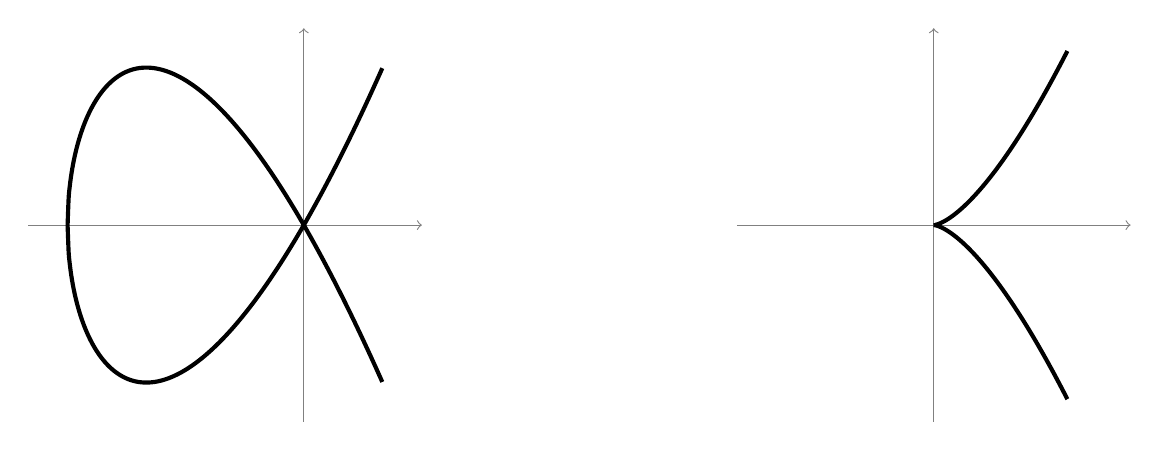
\begin{tikzpicture}
\draw[->,gray] (-3.5, 0) -- (1.5,0);
\draw[->,gray] (0,-2.5) -- (0,2.5);
\draw[domain=-3:1, smooth, samples=300, line width=1.5pt] plot (\x, {sqrt(\x^3 + 3*(\x)^2)}) ;
\draw[domain=-3:1, smooth, samples=300, line width=1.5pt] plot (\x, {- sqrt(\x^3 + 3*(\x)^2)});

\begin{scope}[shift={(8,0)}]
\draw[->,gray] (-2.5, 0) -- (2.5,0);
\draw[->,gray] (0,-2.5) -- (0,2.5);
\draw[domain=0:1.7, smooth, samples=300, line width=1.5pt] plot (\x, {sqrt(\x^3)}) ;
\draw[domain=0:1.7, smooth, samples=300, line width=1.5pt] plot (\x, {- sqrt(\x^3)});
\end{scope}
\end{tikzpicture}

\end{document}